\documentclass[a4paper,oneside,12pt]{book}

%----------------------------------------------------------------------------------------
%	README!
%   Welcome. It's worth having a read through this file
%   to set up the broad parameters, such as the name of
%   the degree, the school/department, the type of work
%   (dissertation/Final Year Project/report, etc. as well
%   as your own details.
%----------------------------------------------------------------------------------------

%----------------------------------------------------------------------------------------
%	COVER PAGE
%   The cover page is laid out in title/title.tex. You can choose a colour
%   or black and white logo
%----------------------------------------------------------------------------------------

%----------------------------------------------------------------------------------------
%	THESIS INFORMATION
%   Put title, author name, degree, type of work, school, department in here
%   It will be used for the title page and for the embedded PDF information
%----------------------------------------------------------------------------------------

\newcommand{\thesistitle}{Title of Work} % Your thesis title, this is used in the title and abstract
\newcommand{\degree}{MAI (Computer Engineering)} % Your degree name, this is used in the title page and abstract
\newcommand{\typeofthesis}{dissertation} % dissertation, Final Year Project, report, etc.
\newcommand{\authorname}{Dara \'O S\'uilleabh\'ain} % Your name, this is used in the title page and PDF stuff
%% Do not put your Student ID in the document, as TCD will not publish
%% documents that contain both your name and your Student ID.

\newcommand{\keywords}{this, that, more} % Keywords for your thesis
\newcommand{\school}{\href{http://www.scss.tcd.ie}{School of Computer Science and Statistics}} % Your school's name and URL, this is used in the title page

%% Comment out the next line if you don't want a department to appear
%\newcommand{\department}{\href{http://researchgroup.university.com}{Department Name}} % Your research group's name and URL, this is used in the title page

\AtBeginDocument{
\hypersetup{pdftitle=\thesistitle} % Set the PDF's title to your title
\hypersetup{pdfauthor=\authorname} % Set the PDF's author to your name
\hypersetup{pdfkeywords=\keywords} % Set the PDF's keywords to your keywords
\hypersetup{pdfsubject=\degree} % Set the PDF's keywords to your keywords
}

%% Language and font encodings
\usepackage[T1]{fontenc} 
\usepackage[utf8]{inputenc}
\usepackage[english]{babel}

%% Bibliographical stuff
\usepackage[round,sort,comma,numbers]{natbib}

%% Document size
% include showframe as an option if you want to see the boxes
\usepackage[a4paper,top=2.54cm,bottom=2.54cm,left=2.54cm,right=2.54cm,headheight=16pt]{geometry}
\setlength{\marginparwidth}{2cm}
%% Useful packages
\usepackage{amsmath}
\usepackage[autostyle=true]{csquotes} % Required to generate language-dependent quotes in the bibliography
\usepackage[pdftex]{graphicx}
\usepackage[colorinlistoftodos]{todonotes}
\usepackage[colorlinks=true, allcolors=black]{hyperref}
\usepackage{caption} % if no caption, no colon
\usepackage{sfmath} %use sans-serif in the maths sections too
\usepackage[parfill]{parskip}    % Begin paragraphs with an empty line rather than an indent
\usepackage{setspace} % to permit one-and-a-half or double spacing
\usepackage{enumerate} % fancy enumerations like (i) (ii) or (a) (b) and suchlike
\usepackage{booktabs} % To thicken table lines
\usepackage{fancyhdr}

\pagestyle{plain} % Embrace simplicity!

%% The Mechanical engineers require your name and ID on the top of every page.
%% Uncomment the following block if you want your name and ID at the top of
%% (almost) every page.

%\pagestyle{fancy}
%\fancyhf{} % sets both header and footer to nothing
%\renewcommand{\headrulewidth}{0pt}
%\cfoot{\thepage}
%\ifdefined\authorid
%\chead{\it \authorname\ (\authorid)}
%\else
%\chead{\it \authorname}
%\fi
%% End of block

%% It is not a requirement of the university that the font should be sans-serif, but
%% the Mechanical engineers require it. Comment out the following line to disable it
\renewcommand{\familydefault}{\sfdefault} %use the sans-serif font as default

%% If you're not using sans-serif, consider using Palatino instead of the LaTeX standard
%\usepackage{mathpazo} % Use the Palatino font by default if you prefer it to Computer Modern

\renewcommand{\theequation}{\arabic{equation}} %% use continuous equation numbers

%% Format Chapter headings appropriately
\usepackage{titlesec}
\titleformat{\chapter}[hang] 
{\normalfont\huge\bfseries}{\thechapter}{1cm}{} 

\title{\thesistitle}
\author{\authorname}

\frontmatter
\begin{document}
\begin{titlepage}

\center % Center everything on the page

%% All the text parameters should be taken from the start of the main.tex file.
%% You should only alter stuff here if you want to change the layout

%----------------------------------------------------------------------------------------
%	LOGO SECTION
%----------------------------------------------------------------------------------------
%% Choose one of the following -- a colour or black-and-white logo


\includegraphics{title/Trinity_RGB_transparent_main.png}\\[1cm] 
%
\includegraphics[width=12cm]{title/black-stacked-trinity.jpg}\\[1cm] 

\Large \school\\[1.5cm] % Minor heading such as course title
\ifdefined\department
\large \department\\[1.5cm] % Minor heading such as course title
\fi

%----------------------------------------------------------------------------------------
%	TITLE SECTION
%----------------------------------------------------------------------------------------
\makeatletter
{ \huge \bfseries \thesistitle}\\[1.5cm] % Title of your document
 

%----------------------------------------------------------------------------------------
%	AUTHOR SECTION
%----------------------------------------------------------------------------------------

\ifdefined\authorid
\authorname\\ % Your name
\authorid\\[2cm] % Your Student ID
\else
\authorname\\[2cm] % Your name
\fi

%----------------------------------------------------------------------------------------
%	DATE SECTION
%----------------------------------------------------------------------------------------

{\large \today}\\[2cm] % Date, change the \today to a set date if you want to be precise

 
%----------------------------------------------------------------------------------------
%	TYPE OF THESIS SECTION
%----------------------------------------------------------------------------------------
\vfill
 A \typeofthesis\ submitted in partial fulfilment\\of the requirements for the degree of\\
\degree

\vfill % Fill the rest of the page with whitespace

\end{titlepage}
\pagenumbering{roman}
\section*{\Huge{Declaration}}
\vspace{1cm}
I hereby declare that this \typeofthesis\ is entirely my own work and that it has not been submitted as an exercise for a degree at this or any other university.

\vspace{1cm}
I have read and I understand the plagiarism provisions in the General Regulations of the University Calendar for the current year, found at \url{http://www.tcd.ie/calendar}.
\vspace{1cm}

I have also completed the Online Tutorial on avoiding plagiarism `Ready Steady Write', located at \url{http://tcd-ie.libguides.com/plagiarism/ready-steady-write}.
\vspace{3cm}

Signed:~\rule{5cm}{0.3pt}\hfill Date:~\rule{5cm}{0.3pt}

\chapter*{Abstract}
A short summary of the problem investigated, the approach taken and the key findings. This should not be more that around 400 words.

The must be on a separate page.

\newpage
\onehalfspacing\raggedright %\raggedright turns off justification and hypenation

\section*{\Huge{Acknowledgements}}
Thanks Mum!

You should acknowledge any help that you have received (for example from technical staff), or input provided by, for example, a company.
\tableofcontents
\listoffigures
\listoftables
\newpage
\section*{\Huge{Nomenclature}}
\begin{tabular}{lp{9cm}l}
A&Area of the wing&$m^{2}$\\
B\\
C& Roman letters first, with capitals\ldots\\
a&then lower case.\\
b\\
c\\
$\Gamma$&Followed by Greek capitals\ldots\\
$\alpha$&then lower case greek symbols.\\
$\beta$\\
$\epsilon$\\
TLA&Finally, three letter acronyms and other abbreviations arranged alphabetically\\
\end{tabular}
\vspace{2cm}

If a parameter has a typical unit that is used throughout your report, then it should be included here on the right hand side.

If you have a very mathematical report, then you may wish to divide the nomenclature list into functions and variables, and then sub- and super-scripts.

Note that Roman mathematical symbols are typically in a serif font in italics.

\mainmatter
\chapter{Introduction}

\chapter{Background}

\chapter{Technical Work}
\label{ch:tw}

%In this chapter we will discuss the experiments and the process that has been followed to develop the model for predicting the amplifier output profile


\section{Introduction} 
\label{tw:intro}

This chapter will discuss the experiments that have been carried out and the process that has been followed leading to the development of a machine learning model capable of predicting the output power spectrum of an EDFA. 
The work that has been undertaken will be split into sections as follows:
\begin{itemize}
    \item Amplifier characterisation, a detailing of the experiments carried out in order to characterise the amplifier model that has been used throughout this thesis.
    
    \item Data generation will discuss the experiment that has been designed to generate suitable training data for the development of the machine learning model.
    
    \item Model Design will outline the development of the baseline machine learning model, the development environment and the design choices made during the development process.
    
    \item Model Refinement 1 – Sensitivity Analysis, will discuss the analysis of the model from section \ref{model_design}. The aim of this analysis is to determine a strategy for reducing the amount of training data required by the ML model.
    
    \item Model Refinement 2 – Pruning and Quantization, will discuss the optimisation methods that have been applied to improve the model in terms of memory requirements, training time and design efficiency. 
\end{itemize}


%%%%%%%%%%%%%%%%%%%%%%%%%%%%%%%%%%
% Beginning of New Section Here
%%%%%%%%%%%%%%%%%%%%%%%%%%%%%%%%%%

\newpage
\section{Amplifier Characterisation}
\label{tw:sec:amp_char}


\subsection{Introduction}
This section will detail the characterisation experiment that was carried out on the amplifier used throughout this project. In place of a physical EDFA amplifier a virtual model from a photonics simulation software package was used. A detailed description of the software package used will also be provided in the following section.	

The need to carry out an experimental characterisation of the EDFA arises from the necessity to verify the accuracy of the virtual model to one of a physical amplifier. This process will determine characteristics of the amplifier, such as the gain profile, the impact of noise on the amplifier output and the amplifier fidelity, in terms of the presence of saturation effects and interaction effects between the various input channels. The results of this characterisation will be used to inform the design of later experiments, and the development of the machine learning model itself.

\subsection{Amplifier model}
An EDFA model from the VPI Photonics software suite (VPI) was used for this experiment. VPI is a photonics design tool, which was specifically suited to the modelling of fibre optics and optical amplifiers. There are a variety of amplifier models available in from the VPI software. 

A black box amplifier, “AmpBlackBoxOpt” will be used throughout this report. It is a model of an EDFA amplifier based on data measured from a physical amplifier. The amplifier output accounts for wavelength-dependent gain and noise spectra. The amplifier operation can be controlled by a set gain value, a set output power value, or can operate in constant saturation mode.

This experiment is to characterise the amplifier model, this is necessary in order to verify that the amplifier will operate as expected under a simulated network traffic load.  The experiment should:

\begin{itemize}    
    \item Determine the output gain profile. This will show whether a gain flattening filter has been applied to the amplifier output.\\

    \item Determine if the amplifier model has a saturation point, and if so what it is.\\
    
    \item Verify that the amplifier model accounts for interaction effects between input channels.\\
\end{itemize}





\subsection{Experimental Setup}
The experimental setup to characterise the amplifier is shown in figure \ref{fig:tw_amp_char}.
The amplifier input consists of 3 optical signal sources multiplexed together:

\begin{figure}
    \centering
    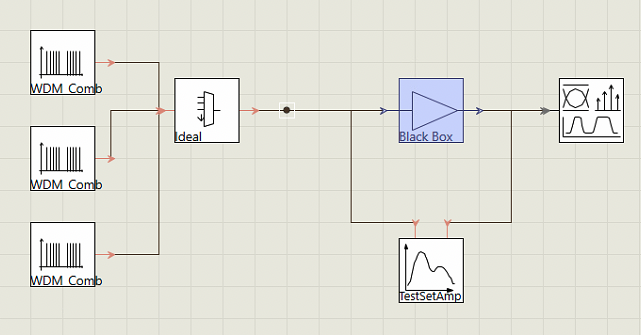
\includegraphics[width=\linewidth]{images/technical_work/section_1_characterisation/amp_char_ex_setup.png}
    \caption{Experimental Setup in VPI}
    \label{fig:tw_amp_char}
\end{figure}


\begin{enumerate}
    \item The primary input source, the generated by a WDM comb module outputting 44 channels spaced in 100GHz intervals, over the range: 192.05THz - 196.45THz. This frequency range and spacing was chosen as it matched the frequency spacing of the ITU DWDM frequency grid. The output channel power was set at 50$\mu$W as to emulate a realistic input to an EDFA that might occur in an actual network scenario. \\
    
    \item The lower variable source, this optical source will output a single channel at a frequency of 192.535THz, the output power of the signal will be varied during the course of the experiment.\\
    
    \item The upper variable source will mirror the lower variable source at a frequency of 195.935THz and will also be varied during the course of the experiment.  
\end{enumerate}


The three signal sources are combined using an ideal multiplexer and inputted to the black box amplifier. The output of the amplifier was sent to an optical signal analyser to be graphed.

The output powers of the lower and upper sources were varied from a value of 1$\mu$W to 1W in 5 steps. Only optical signal from either source was active during a given step.

\subsection{Results}


The results of the experiment can be seen in figures \ref{fig:tw_amp_char_lc} and \ref{fig:tw_amp_char_uc} , where the output spectrum as a result of varying the lower source is shown in figure and as a result of varying the upper source is shown in figure. 

From the figures it can be clearly seen that the output spectrum of the amplifier is non-flat. By examining the change in the output spectrum as the two sources are varied the interaction effects between channels can be seen. The higher frequency channel has a much greater impact on the overall output spectrum than the lower frequency channel of the same power. The gain of the entire output spectrum is suppressed as the power of the high frequency channel is increased. Whereas increasing the power of the lower frequency channel results in a marginal increase in the output spectrum. 



\renewcommand{\arraystretch}{0.5}
\begin{figure}
    \floatpagestyle{empty}
    \centering
    \caption{Shows the effect the power of the lower channel has on the gain spectrum.}
    \begin{tabular}{c}
        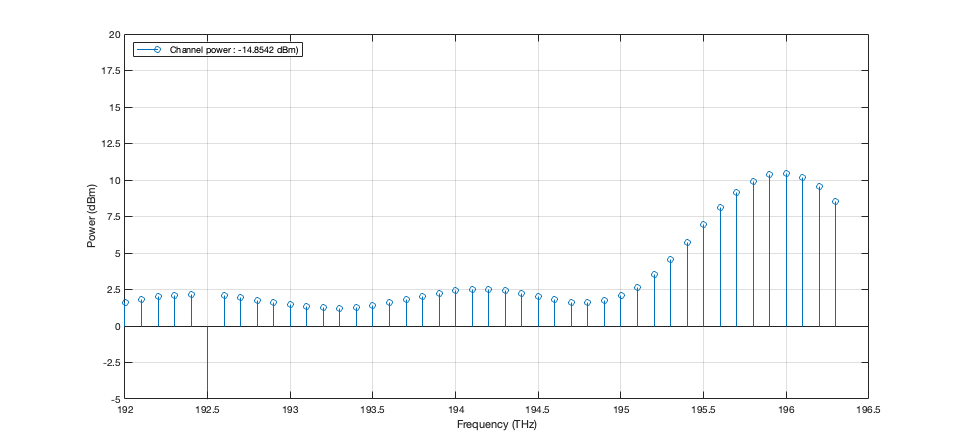
\includegraphics[width=0.85\textwidth]{images/technical_work/section_1_characterisation/figures/1.png} \\
        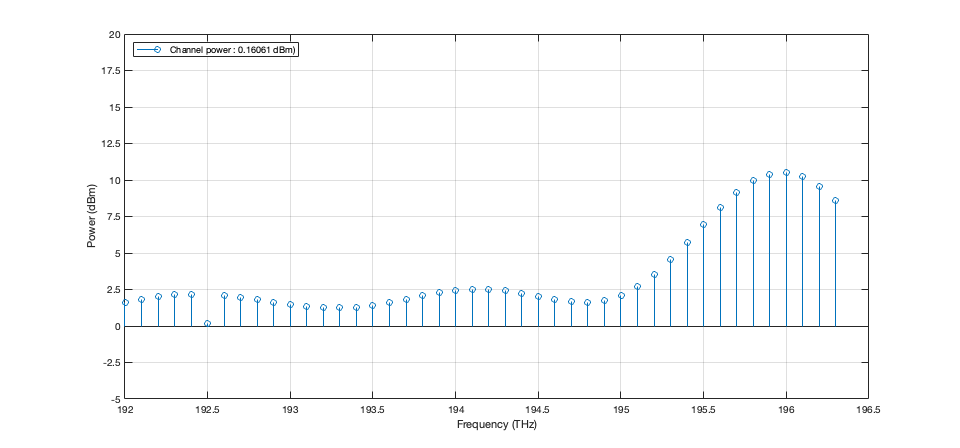
\includegraphics[width=0.85\textwidth]{images/technical_work/section_1_characterisation/figures/2.png} \\
        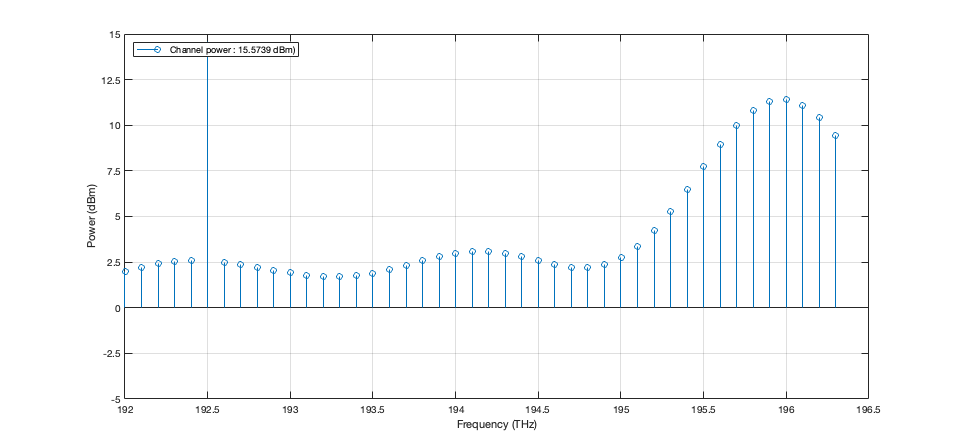
\includegraphics[width=0.85\textwidth]{images/technical_work/section_1_characterisation/figures/3.png} \\
        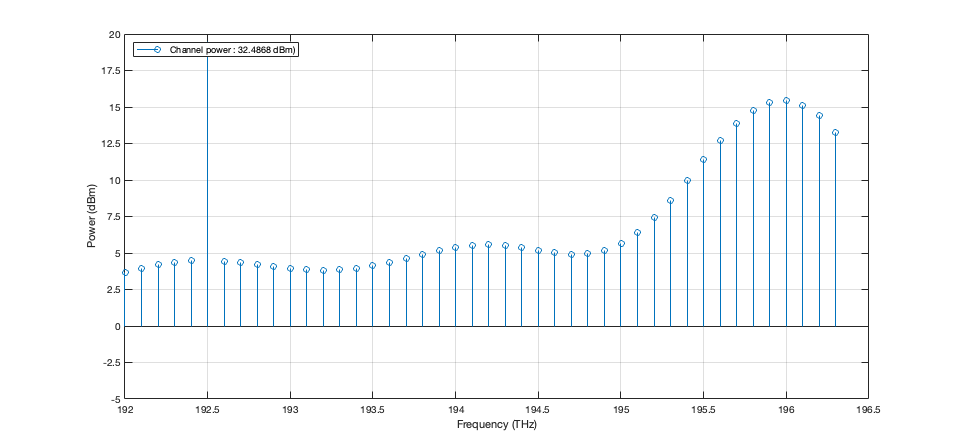
\includegraphics[width=0.85\textwidth]{images/technical_work/section_1_characterisation/figures/4.png} \\
    \end{tabular}
    \label{fig:tw_amp_char_lc}
\end{figure}

\begin{figure}
    \floatpagestyle{empty}
    \caption{Shows the effect the power of the upper channel has on the gain spectrum.}
    \centering
    \begin{tabular}{c}
        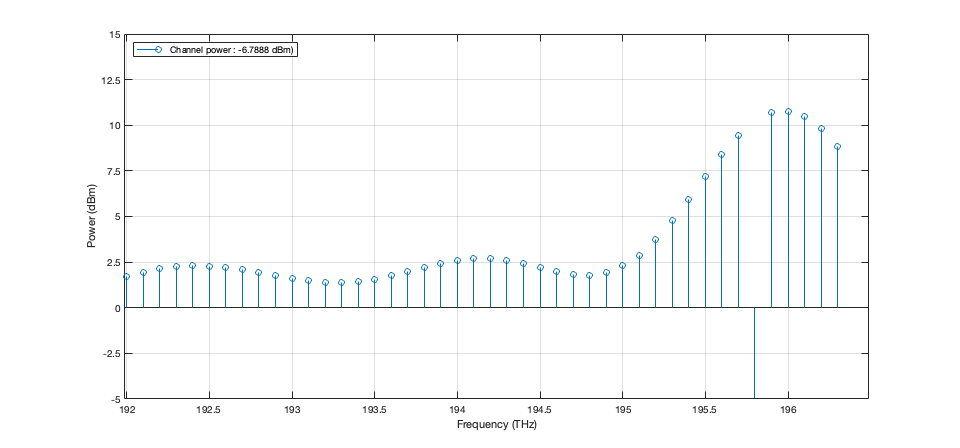
\includegraphics[width=0.85\linewidth]{images/technical_work/section_1_characterisation/figures/6.png} \\
        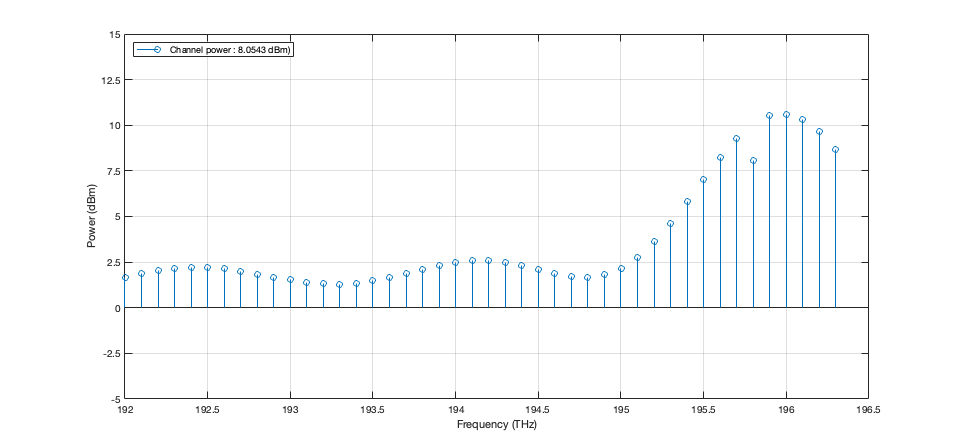
\includegraphics[width=0.85\linewidth]{images/technical_work/section_1_characterisation/figures/7.png} \\
        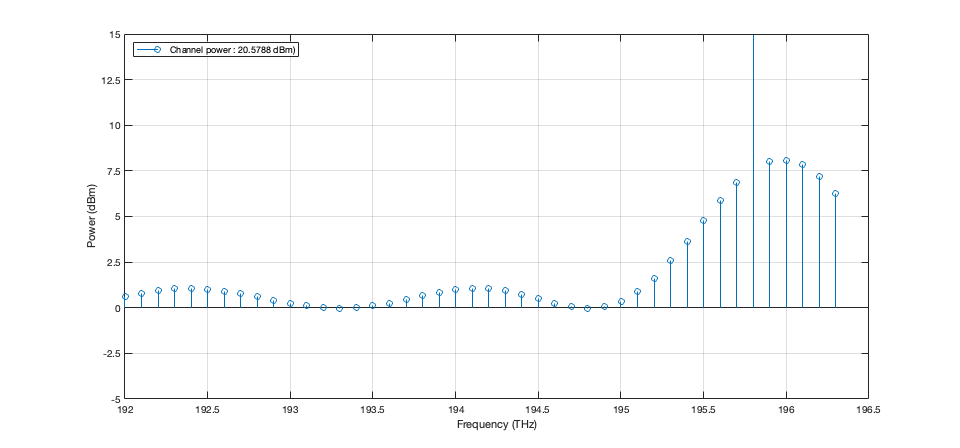
\includegraphics[width=0.85\linewidth]{images/technical_work/section_1_characterisation/figures/8.png} \\
        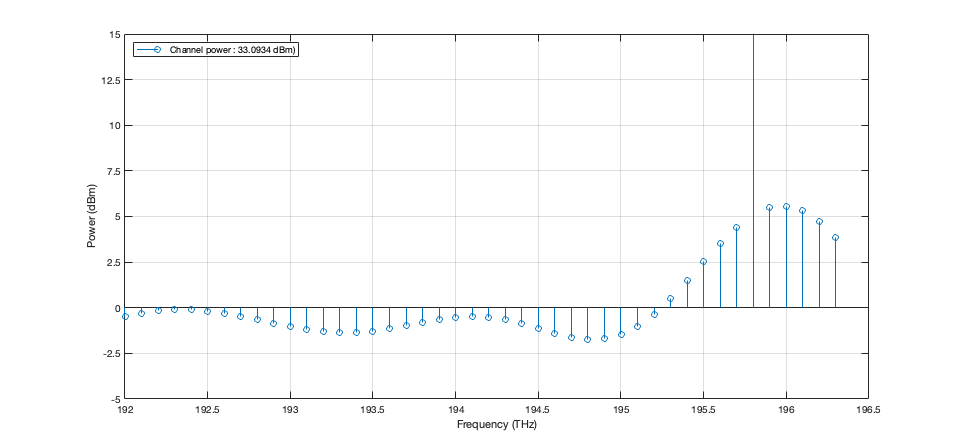
\includegraphics[width=0.85\linewidth]{images/technical_work/section_1_characterisation/figures/9.png} \\
    \end{tabular}
    \label{fig:tw_amp_char_uc}
\end{figure}



\FloatBarrier
\subsection{Conclusion}


%%%%%%%%%%%%%%%%%%%%%%%%%%%%%%%%%%
% Beginning of New Section Here
%%%%%%%%%%%%%%%%%%%%%%%%%%%%%%%%%%


\newpage
\section{Data Generation Experiment}
\label{tw:sec:data_gen}

\subsection{Introduction}

In this section  the experiment used to generate training data for the ML model will be discussed. The training data must emulate optical signal traffic from real world scenarios to provide the model with sufficient data to be able to predict the outputs of actual amplifiers used in optical networks.

The ITU define a frequency grid for DWDM applications centred at 193.1 THz and using channel spacings up to 100GHz. This frequency range from 1530nm (195.943THz) to, 1565 (191.561THz), known as the C band in fibre optic communications. The C band is the primary wavelength used for long distance optical communication, as it is in this frequency band that fibre optic cables have lowest losses. 

The channel spacing was set at 100GHz to conform to the standard ITU DWDM frequency grid. A common channel plan found in many DWDM systems is to use 44 channels spaced at 100GHz or 88 channels spaced at 50GHz. In this case 44 channels will be used.  

The channel power was set at 50$\mu$W, as this is reflective of a typical channel input power for an EDFA in an optical communication network. The channel power was not varied between channels.

Maintaining a constant channel power has several implications for the model that will be trained on this data. As a result of applying this restriction the model will not account for cases where the power of all channels is varied form 50[mu]W, or where the channel powers are not uniform. 

This restriction will reduce variability in the training data and enable the model to learn the effects of different channel loading conditions more easily. The impact that channels have on each other will be solely due to their relative frequency, as opposed to their relative power, and relative frequency.


Each training data sample will consist of two arrays, both 44 units long. The array of input powers randomly generated by the VPI simulator and, the corresponding array of output powers measured from the output of the amplifier. The training samples can vary in the following ways:
\begin{itemize}
    \item The input power of each of the 44 channels will either be 0W or 50$\mu$W. The number and location of the nonzero channels will be randomly set.
    
    \item The output powers will either be, 0$\mu$W if the input power of that channel was 0$\mu$W, or will be some non-zero value of power determined by the channel specific gain.
\end{itemize}

The gain of each channel will depend on the channel loading conditions, i.e., which channels are on and the relation between a given channel and all other “on” channels.




\subsection{Experimental Setup}
\FloatBarrier

\begin{figure}
    \caption{Experimental setup in VPI. Figure \ref{fig:tw:top_lvl} shows the top level simulation. Figure \ref{fig:tw:co_sim_galaxy} shows the expanded co-simulation sub-module, referred to as a galaxy.}
    \begin{subfigure}{\textwidth}
        \centering
        \caption{From left to right, the co-simulation galaxy, EDFA amplifier and the optical systems analyser.}
        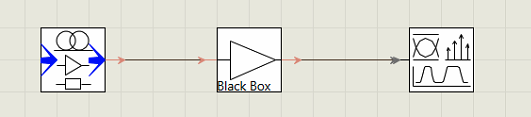
\includegraphics[width=0.8\textwidth]{images/technical_work/section_2_data generation/ex_setup.png}
        \label{fig:tw:top_lvl}
    \end{subfigure}
    \begin{subfigure}{\textwidth}
        \centering
        \caption{Expanded co-simulation galaxy, showing the co-simulation model being used as an output.}
        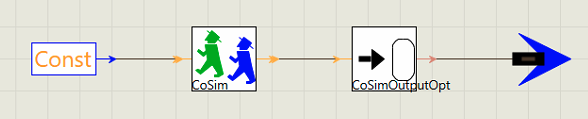
\includegraphics[width=0.8\textwidth]{images/technical_work/section_2_data generation/co_sim_galaxy.png} 
        \label{fig:tw:co_sim_galaxy}
    \end{subfigure}
    \label{fig:tw:exp_setup}
\end{figure}


The experimental setup to generate the training data is shown in figure \ref{fig:tw:exp_setup}. The experiment will generate a random channel loading scenario. A random number of channels $n$, between 2 and 44 inclusive, will be turned “on” i.e., have an input power of 50[mu]W. The frequency of each “on” channel will also be randomly decided. The scenario where the input is a single channel will be ignored. As in this case the single channel will not be impacted by the presence of any other channels.

The $n$ channels will be inputted to the amplifier. The value of the corresponding $n$ output channels along with the $n$ input channels will be recorded. This process will be repeated several thousand times to generate sufficient data to train the ML model. 

As in the experiment from section \ref{tw:sec:amp_char}, the amplifier model from VPI will be used. However, there is no straightforward method to generate a random array of channels in VPI. As such the array of input channels will be generated using MATLAB and then be read into VPI using the simulators co-simulation function.

As seen in figure \ref{fig:tw:exp_setup} the experimental setup consists of setting the output of the MATLAB co-simulation module as the input to the optical amplifier, and measuring the output of the optical amplifier using the optical systems analyser module. 


\subsubsection{MATLAB Channel Generation}

Though the optical channels are generated in MATLAB, for them to be read by VPI they must conform to the internal structure that VPI has defined for optical signals. 

Optical signals in VPI are comprised of noise bins, sampled bands, and parameterised signals, all three signal components must be created for a signal to be used in VPI. 
For the purposes of this experiment, we are only interested in the parameterised signals.

The VPI optical signal components are represented by cell arrays in MATLAB, a cell array for each component will be created, but only the parameterised signal cell array will contain the values of our channels.  

The MATLAB code used to generate the channels can be found in appendix [ref].

The MATLAB script is run each time a training sample is generated. Before a sample is generated the random number generator used to select the channels is re-initialised using the current time. This ensure that the channels generated are indeed random and independent from each other. 



\subsubsection{Verification}

A verification script was created to ensure that the channel generation scrip was functioning as expected.

The verification script records the output of the channel generator over a number of runs and plots the results. The results of performing 5000 runs can be seen in figures \ref{fig:tw:data_gen:rel_ch} and \ref{fig:tw:data_gen:rel_num_ch}. 

As can be seen from the figures there is no bias towards any particular channel nor towards a particular number of channels. The variation in the relative occurrence of the channels and the number of channels generated can be attributed to the number of dummy runs that were produced and is expected to decrease were the number of runs increased. Ensuring that there are no biases in the underlying data used to train the model is critical. Further discussion on this are can be found in section [ref]. The script used to verify the channel generator can be found in appendix [ref].
\begin{figure}
    \centering
    \caption{Results of 5000 dummy runs of the channel generator.}
    \label{fig:tw:dummy_runs}
    \begin{subfigure}{0.49\textwidth}
        \centering
    \caption{Plot of the relative occurrence of each channel.}
    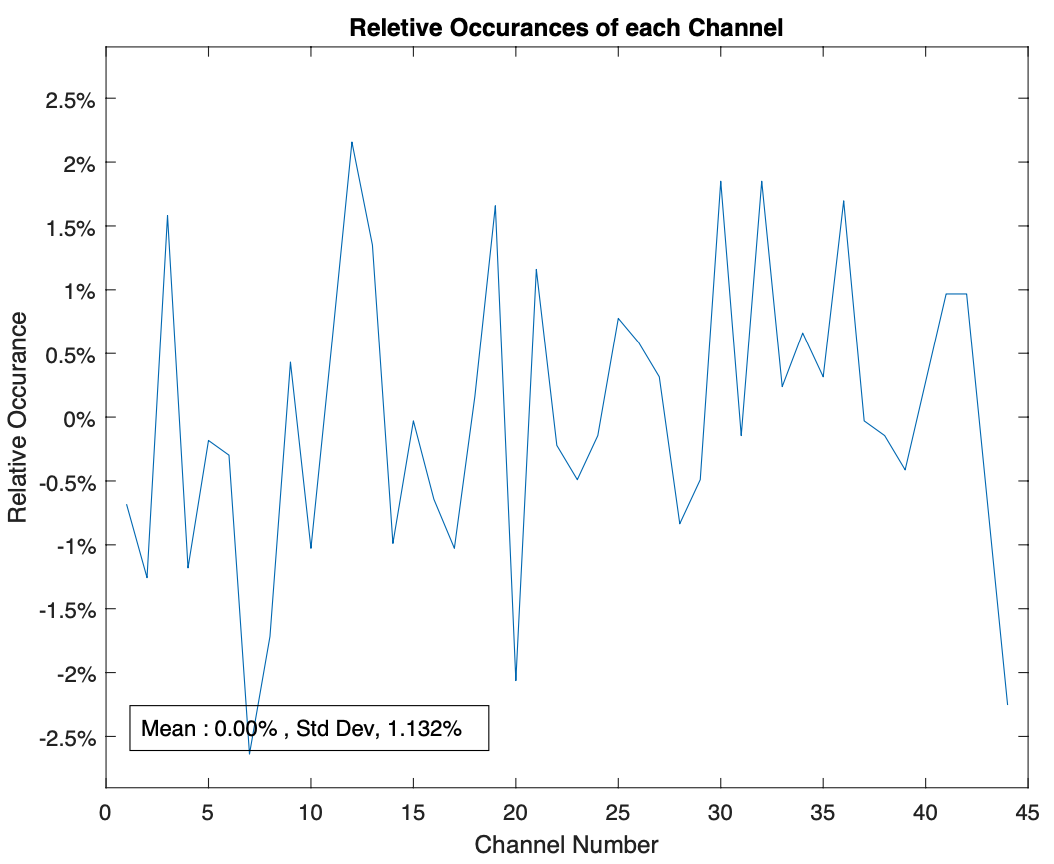
\includegraphics[width=\textwidth]{images/technical_work/section_2_data generation/rel_occur_ch.png}
    \label{fig:tw:data_gen:rel_ch}    
    \end{subfigure}
    \begin{subfigure}{0.49\textwidth}
        \centering
        \caption{Plot of the relative occurrence of the number of channels generated, note the y-axis i scaled by $1e^{-3}$.}
        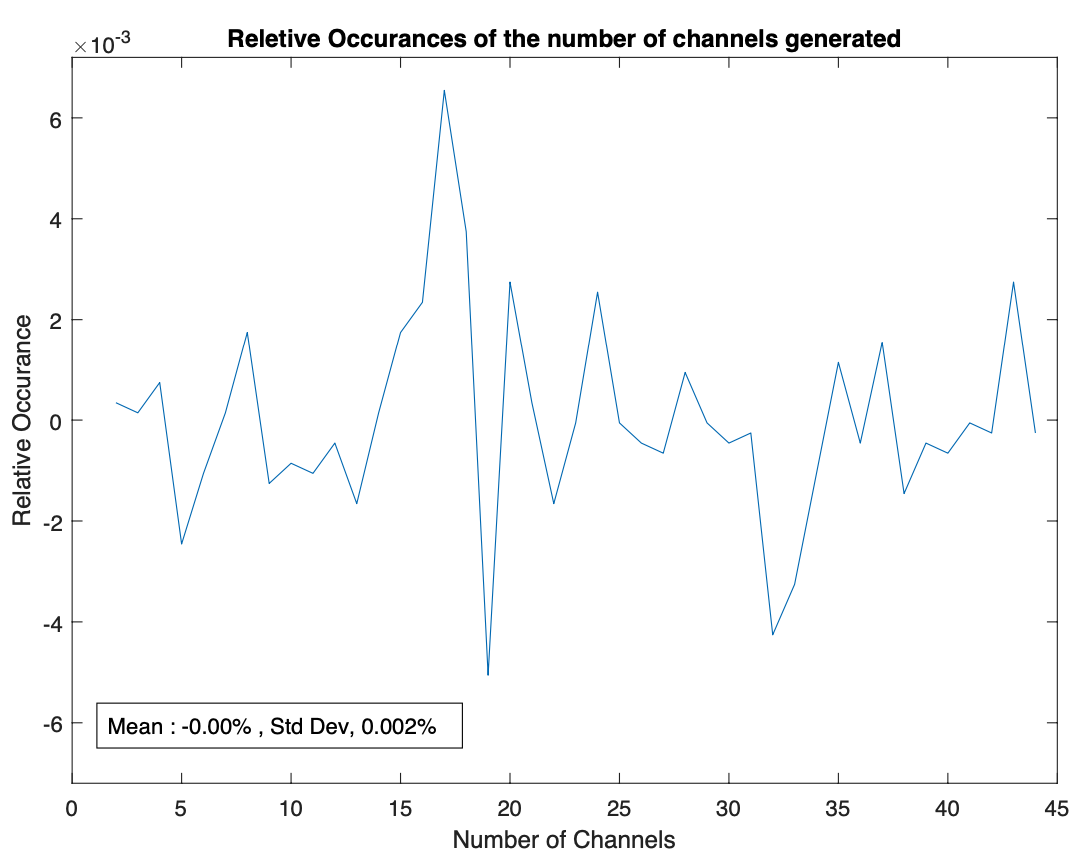
\includegraphics[width=\textwidth]{images/technical_work/section_2_data generation/rel_occur_num_ch.png}
        \label{fig:tw:data_gen:rel_num_ch}
    \end{subfigure}
\end{figure}


\FloatBarrier

\subsection{Results}

A sample of the outputs from the runs of the simulator can be seen in figure \ref{fig:tw:vpi_samp_op}. In figure \ref{fig:tw:vpi_50_op} the variation in the outputs of the channels can be seen. The variation is a result of the impact that different channel loading conditions have on the amplification of each channel.

\begin{figure}[!h]
    \centering
    \caption{Sample outputs from the VPI simulator.}
    \label{fig:tw:vpi_samp_op}
    \begin{subfigure}{\textwidth}
        \centering
        \caption{One sample run from the simulation.}
        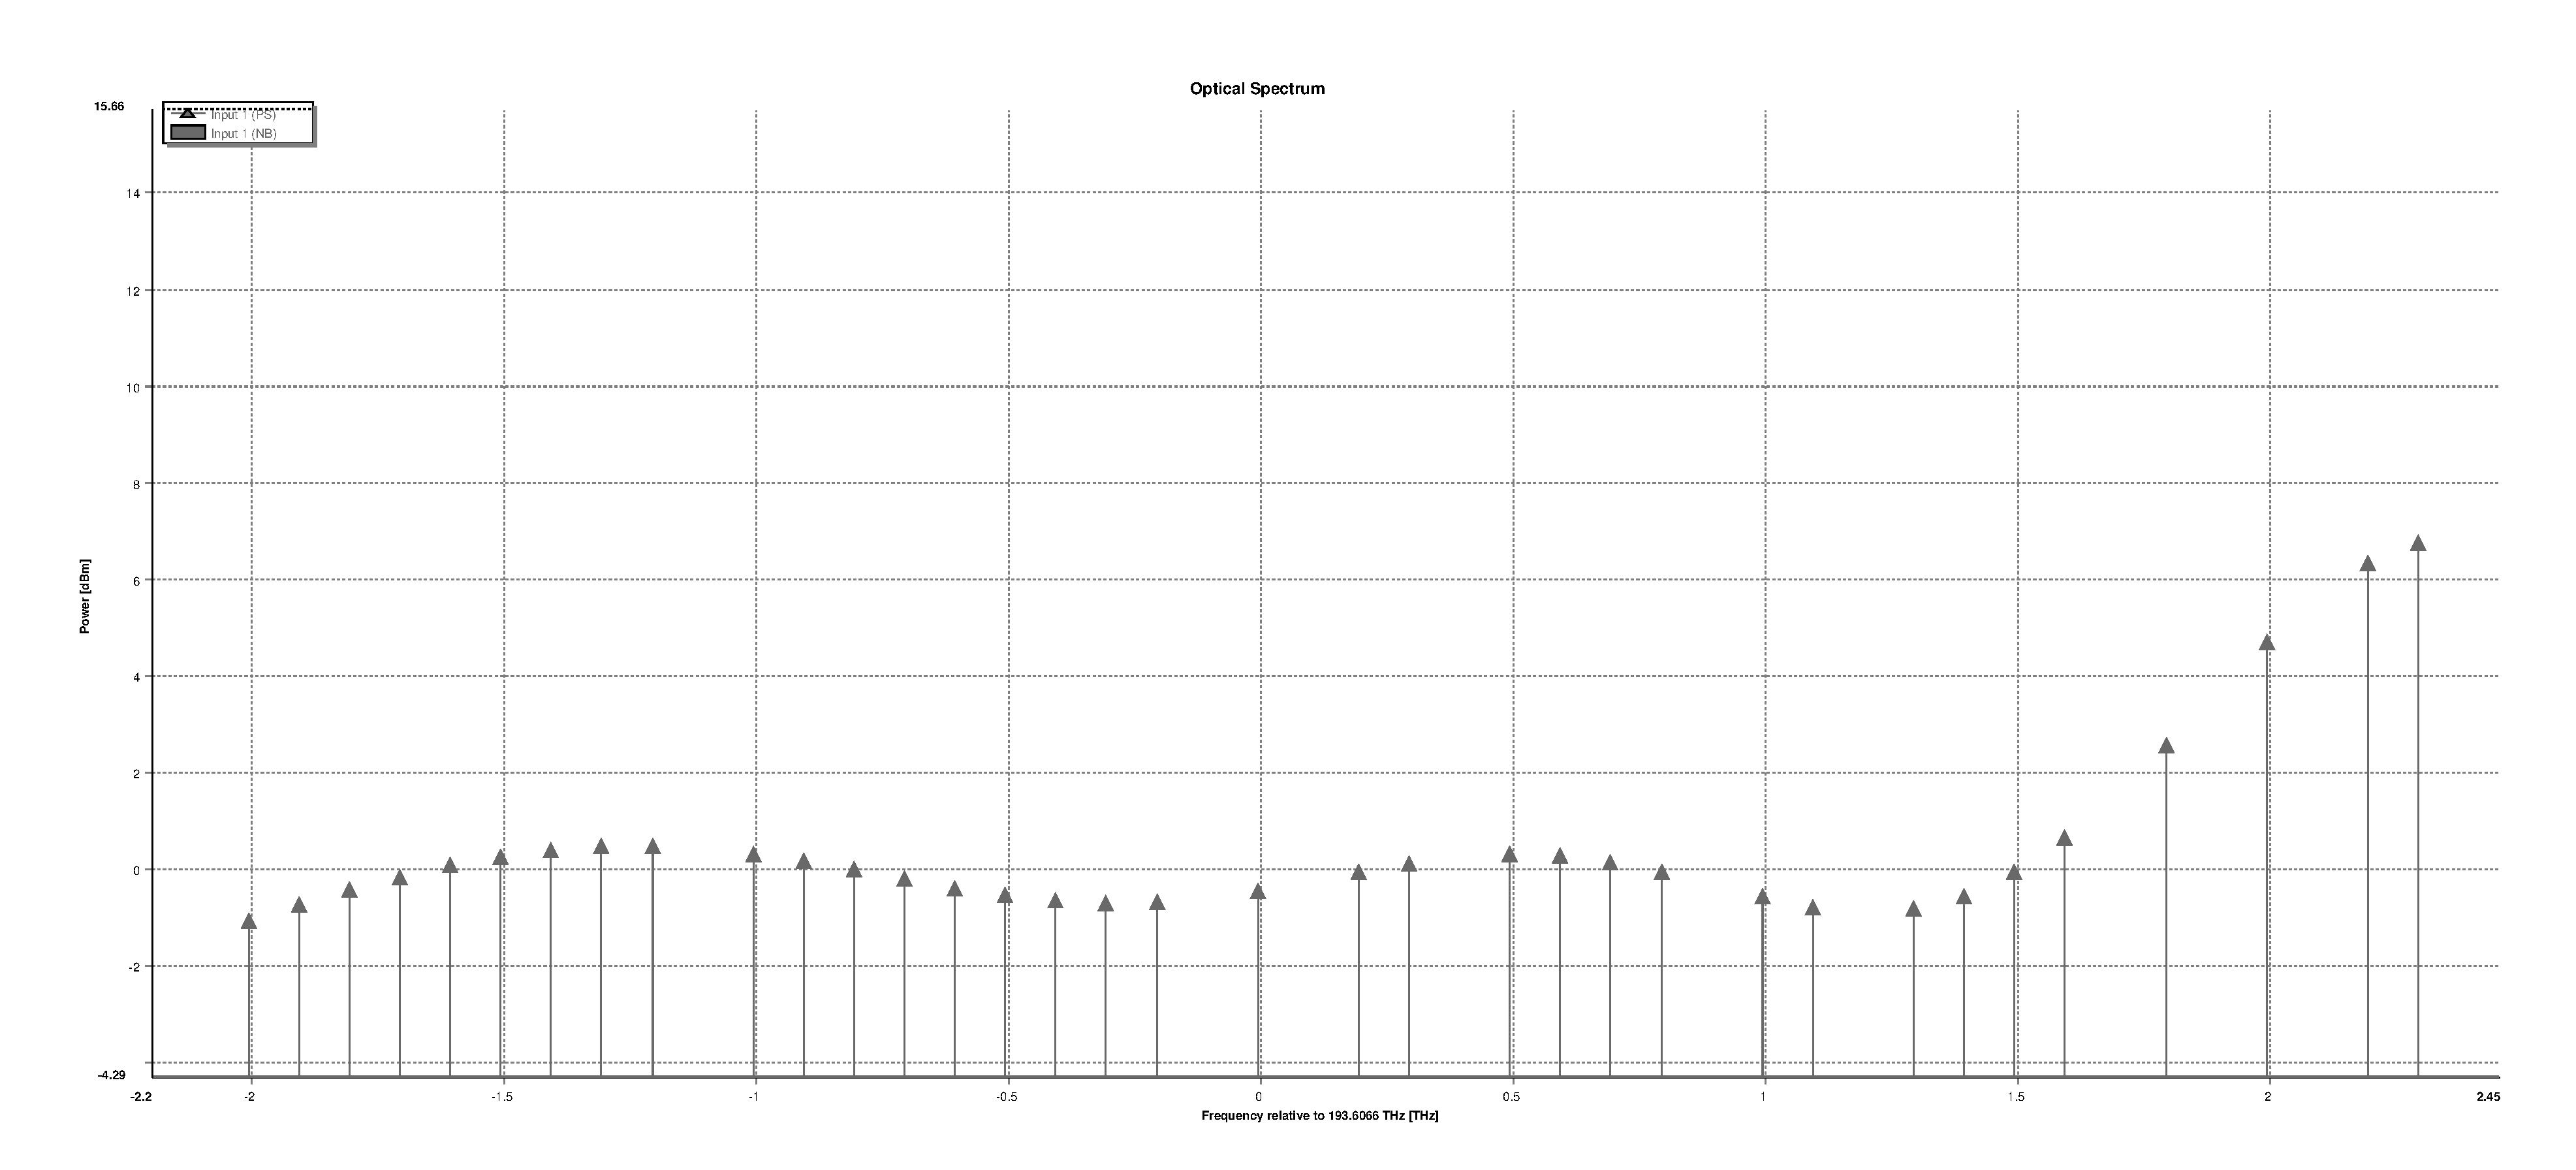
\includegraphics[width=\textwidth]{images/technical_work/section_2_data generation/sample_output_1.pdf}
        
        \label{fig:tw:vpi_1_op}
    \end{subfigure}
    
    \begin{subfigure}{\textwidth}
        \centering
        \caption{A sample of 50 runs from the simulation superimposed on-top of each other. The different runs can be determined by the colouring of the stem in the stem plot.}
        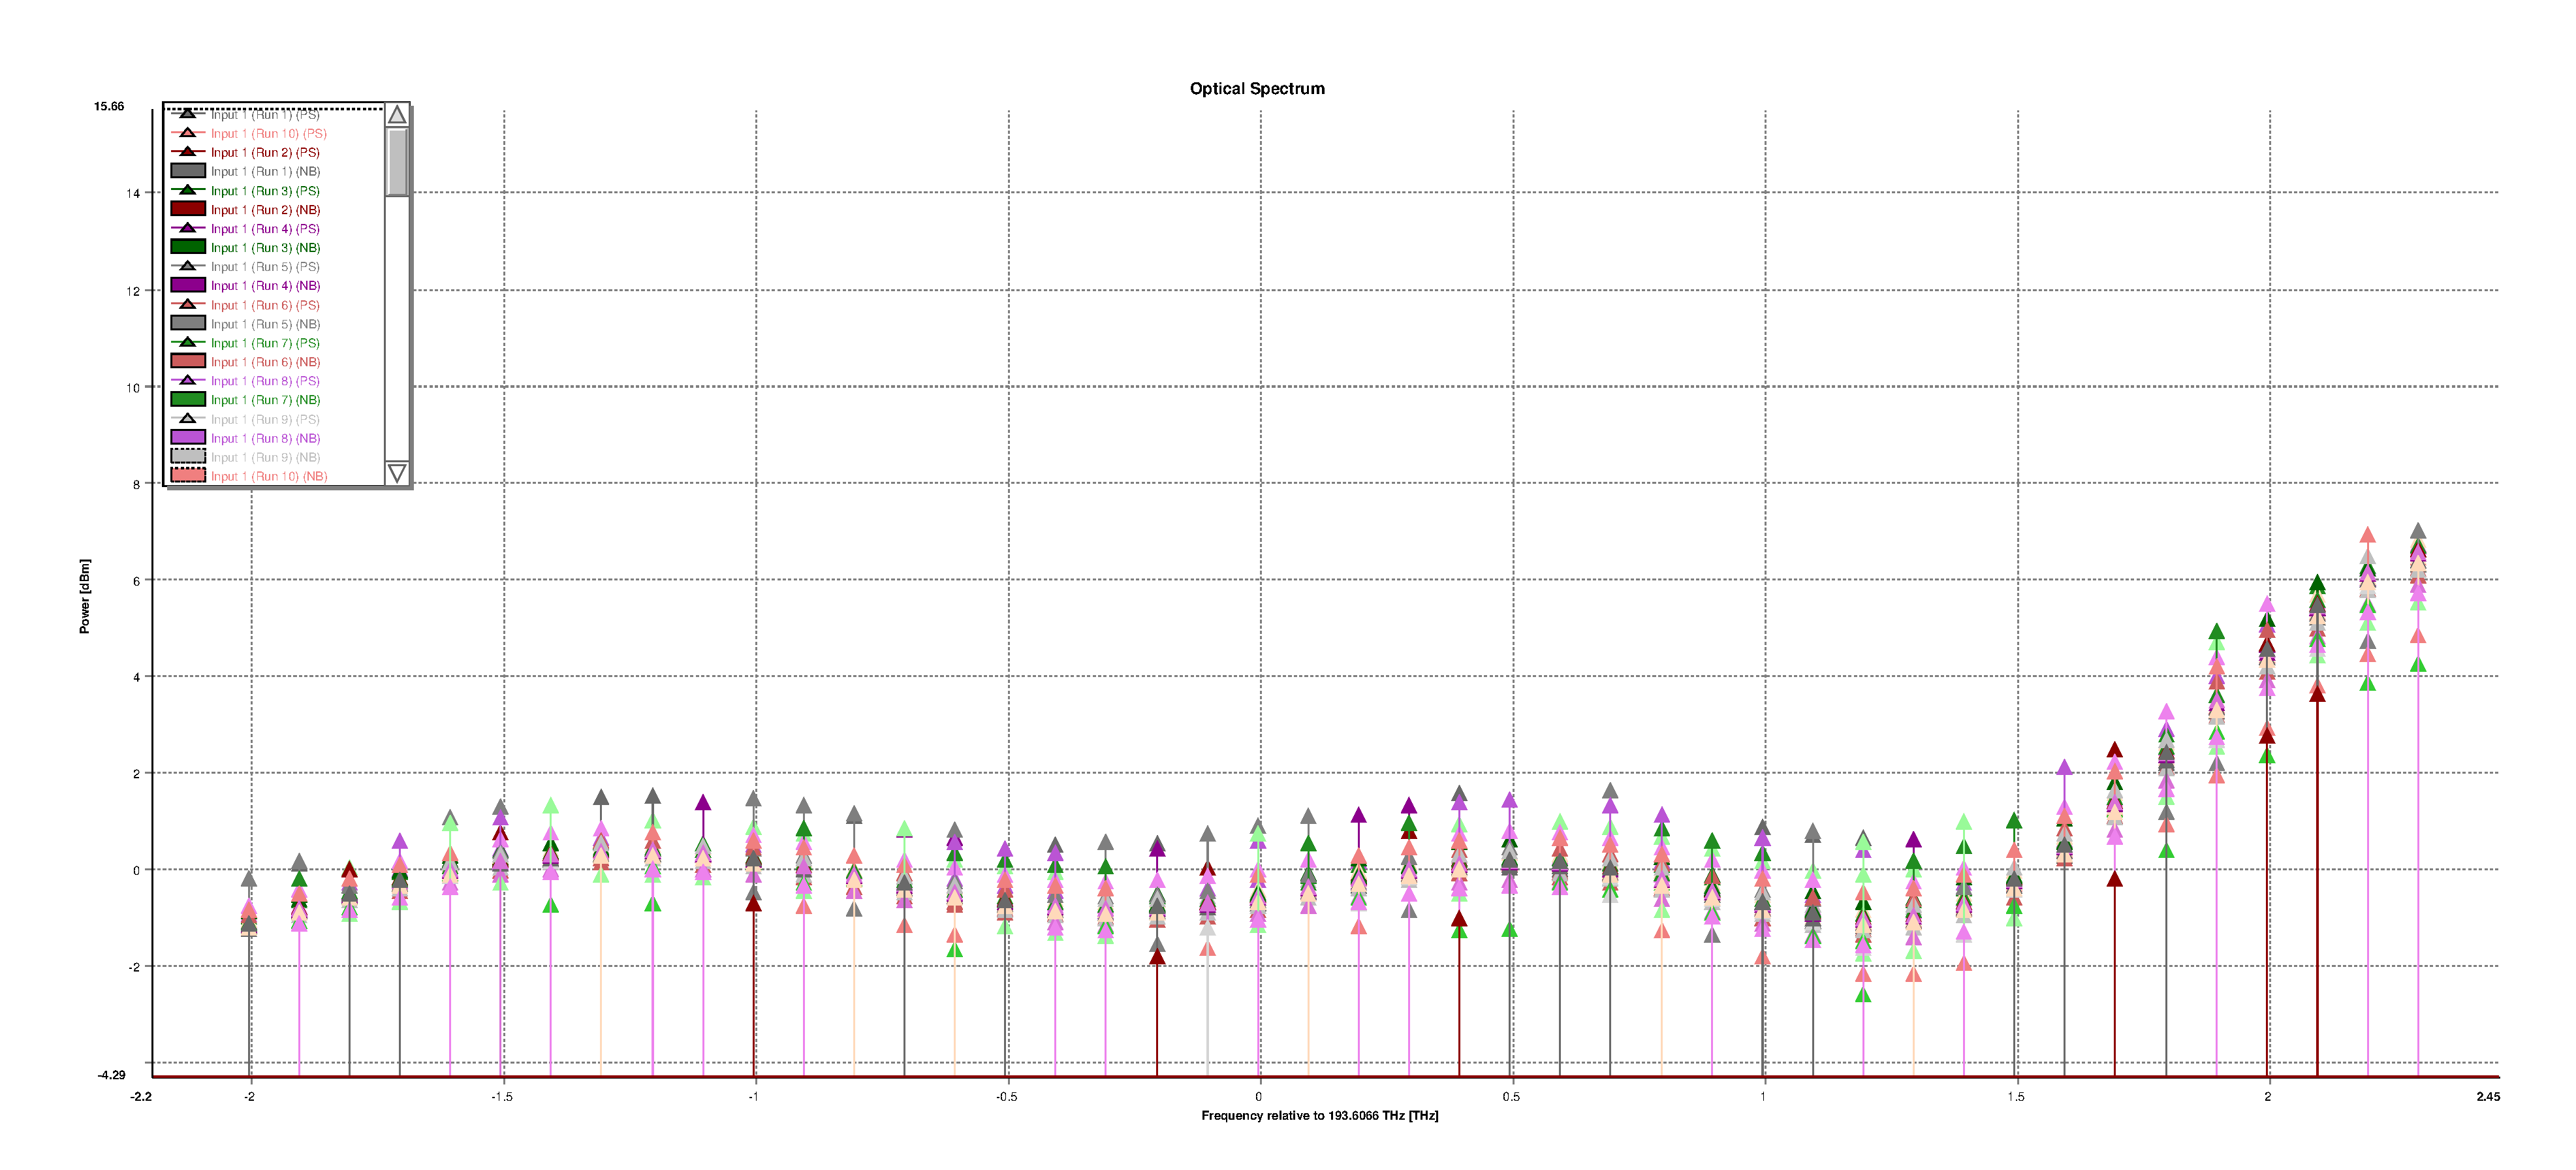
\includegraphics[width=\textwidth]{images/technical_work/section_2_data generation/sample_output_50.pdf}
        
        \label{fig:tw:vpi_50_op}
    \end{subfigure}
\end{figure}
\FloatBarrier
\subsection{Conclusion}


%%%%%%%%%%%%%%%%%%%%%%%%%%%%%%%%%%
% Beginning of New Section Here
%%%%%%%%%%%%%%%%%%%%%%%%%%%%%%%%%%



\newpage
\section{Machine Learning Model}\label{tw:ml_model}


\subsection{Introduction}
In this section the development of the machine learning model will be discussed. The aim of the model is to predict the output power of each channel based on input power. To this end a fully connected neural network will be used. The model was developed using the Tensorflow and Keras Python libraries.

Experiments were carried out to evaluate the performance of 2 different neural networks (NNs) on this regression problem.

Initially a NN with a combined network architecture was developed. This is where the input to the network will be a vector 44 units long, each unit corresponding to the input power of a channel. The output of the network will again be a vector with the 44 output powers of each channel.

Subsequently a model with a discrete network architecture was developed. In this case 44 different neural networks were trained, each network taking the same input vector of the 44 channel powers but instead will be responsible for predicting the output power of a single channel. As the gain each channel receives will be slightly different, the weights of the network will reflect this begin slightly different in each of the 44 networks.


This chapter will be broken down into the following sections:
\begin{enumerate}
    \item Data
    \item Combined Network
    \item Discrete Network
    \item Optimiser
    \item Loss function
\end{enumerate}

\subsection{Data}\label{subsec:ml_model:data}
\FloatBarrier
% Need to include a section about data cleaning 

% Need to include a section about using uW instead of dBM 
% Be good to include a graph of the average output power to show the variation


Training data was generated following the process discussed in section \ref{tw:sec:data_gen}. Using this method 12,000 data samples were generated. The training data must first be formatted before it can be used to train the NN. %should I be saying noise or ASE spontaneous noise here
All channel powers were converted from $dBm$ to $\mu W$ and any noise signals must also be removed from the output spectrum. 

A training validation split of 80:20 was used. A different testing data set of 400 samples was generated for each channel. 

The input power can have a value of either $0\mu W$ or $50 \mu W$, these powers were converted to binary values, or 0 or 1 when using the data to train the NN. It was found that specifying the input as binary values lead to faster model convergence.
A typical training sample can be seen in figure \ref{tab:ex_data_sample}.

% Need to add in graphs showing the faster convergence of the models using binary values as the inputs

\renewcommand{\arraystretch}{1.15}
\begin{table}[!h] 
    \centering
    \caption{Example training sample}
    
    \begin{tabular}[t]{l l l l l l l l }
        \textbf{Channel} & 0 & 1 & 2 & ... & 41 & 42 & 43 \\
        \hline
        \textbf{Frequency (THz)} & 191.6 & 191.7 & 191.8 & ... & 195.6 & 195.7 & 195.8 \\
        \hline
        \textbf{Input} & 1 & 0 & 1 & ... & 0 & 0 &	1 \\
        \hline
        \textbf{Output Power ($\mu W$)} & 1.370 & 0 & 1.656 & ... & 0 &	0 &	19.664 \\
        \hline
    \end{tabular}
    \label{tab:ex_data_sample}
\end{table}

\FloatBarrier
\subsection{Combined Model} \label{sub:sec:comb_mod}
% need to mention where this model can be found, like in what notebook or whatever

\subsubsection{Development}

% Need to insert graph of the model
% Or maybe add in a table like the model summary from keras

A ML model with 44 input features, 4 hidden layers with 1056, 1056, 1056 and 528 neurons respectively and an output layer of 44 units was created. The activation functions of the layers alternated between rectified linear (ReLu) and linear activation.  Dropout of 0.45 was applied after each of the hidden layers.


%Can make table look nicer, add a layer number col and have the words on top of each other on the first row
\begin{table}[!h]
    \centering
    \caption{Combined Model Structure}
    \begin{tabular}{l l l l l l }
        \textbf{Layer} & \textbf{Type} & \textbf{Shape} & \textbf{Parameters} & \textbf{Activation} & \textbf{Dropout Rate} \\
        \hline
        0 & Input & 44 & - & - & - \\
        \hline
        \multirow[t]{2}{*}{1} & Dense & 1,056 & 47,520 & ReLu  & - \\ \cline{2-6}
        
        & Dropout & 1,056 & - & - & 45\% \\
        \hline
        \multirow[t]{2}{*}{2} & Dense & 1,056 & 1,116,192 & Linear  & - \\  \cline{2-6}
        
        & Dropout & 1,056 & - & - & 45\% \\
        \hline
        \multirow[t]{2}{*}{3} &  Dense & 1,056 & 1,116,192 & ReLu  & - \\ \cline{2-6}
        
        & Dropout & 1,056 & - & - & 45\% \\
        \hline
        \multirow[t]{2}{*}{4} & Dense & 528 & 558,096 & Linear  & - \\ \cline{2-6}
        
        & Dropout & 528 & - & - & 45\% \\
        \hline
        5 &Output & 44 & 23,276 & ReLu & - \\
        \hline
    \end{tabular}
    \label{tab:combined_model_struct}
\end{table}

The model was trained using mini-batch gradient decent and the Nadam optimiser to minimise the mean squared error (MSE). A batch size of 512 and a learning rate of $4e^{-5}$ was used.


\subsubsection{Results}
\FloatBarrier

%Need to evaluate what the R-squared metric will mean

The results of training the model for 950 epochs can be seen in figure \ref{fig:ml_model:nn_training}. After 950 epochs the training MSE loss was = 0.2898 and the validation MSE loss was = 0.0556. When evaluating the model on the test set the test loss MSE was = 0.0487. 

\begin{figure}
     \centering
     \caption{Neural Network Training Log}
     \begin{subfigure}[b]{\textwidth}
         \centering
         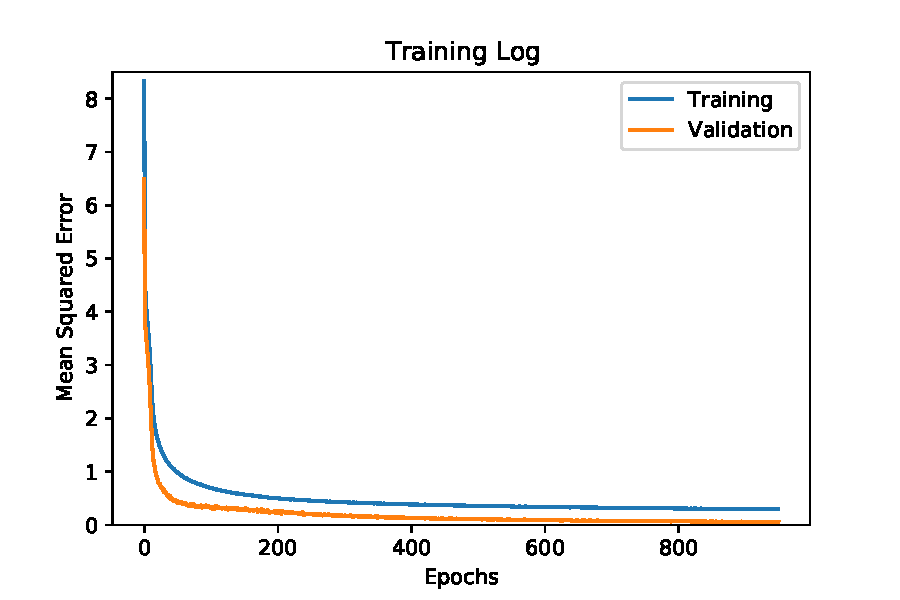
\includegraphics[width=\textwidth]{project/img/ml_model/combined/combined_training_log.pdf}
     \end{subfigure}
     \begin{subfigure}[b]{\textwidth}
         \centering
         \caption{Epochs 100 to 950.}
         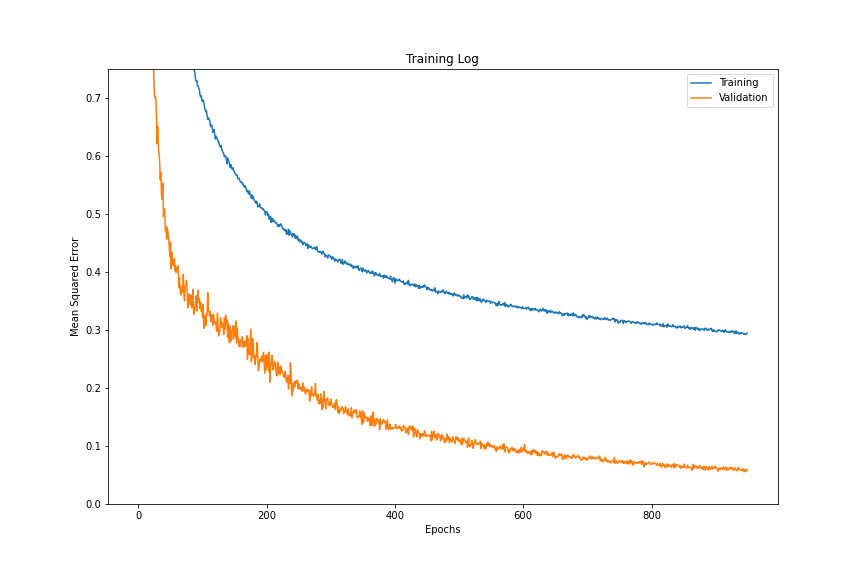
\includegraphics[width=\textwidth]{project/img/ml_model/combined/combined_training_log_inset.png}
         
     \end{subfigure}
        \label{fig:ml_model:nn_training}
\end{figure}





The test loss value is calculated as the MSE between the predicted and actual output vectors. Which is equivalent taking the average of the MSE over all output channels. Due to the disparity between the relative powers of the lower and higher frequency channels the MSE metric under-represents the error on the lower frequency channels. This can be seen in figure \ref{fig:ml_model:pct_err_freq} where the percentage error is graphed against the channel frequency.

A solution to this could be to use the percentage error as the loss metric, however this option is also problematic. As the true output value can be $0\mu W$ in this case any small error in absolute terms between the predicted and true values will result in an extremely large percentage error.

\begin{figure}[!h]
    \centering
    \caption{Test Set percentage Error varying from Channel 1 (191.9 Thz) to Channel 43 (195.7 THz)}
    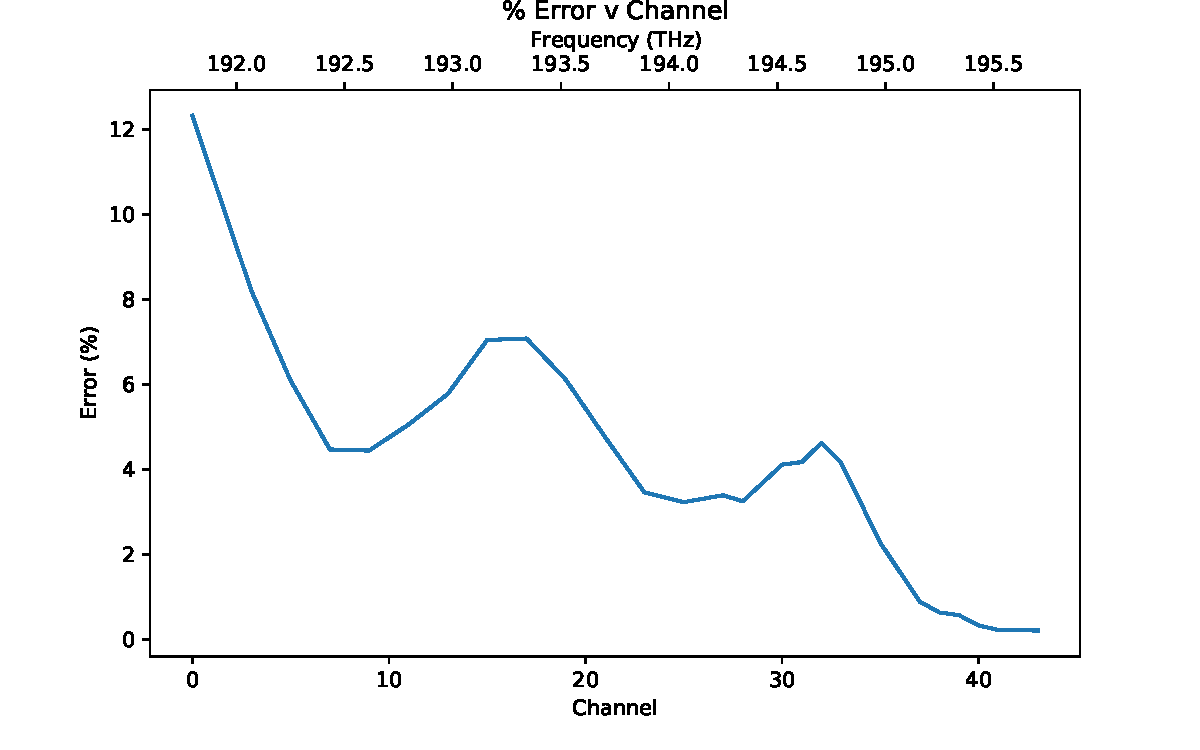
\includegraphics[width = \textwidth]{project/img/ml_model/combined/pct_err_freq.pdf}
    \label{fig:ml_model:pct_err_freq}
\end{figure}

The loss metric should be robust to training samples with $0\mu W$ values while also allowing for the uniform minimising of error over the entire frequency spectrum. 



\FloatBarrier
\subsection{Discrete Model} \label{sub:sec:disc_mod}
% need to mention where this model can be found, like in what notebook or whatever

This model is comprised of 44 distinct NNs where each network will predict the output power of a single channel. The MSE will be used as the loss function for each network, as it is robust to errors in training samples where the true value is $0\mu W$ and due the output being a single neuron the relative difference between channel powers will no longer be an issue.


\subsubsection{Data}
The same training data set from section \ref{subsec:ml_model:data} was used. The NNs output layer is no longer a vector of 44 output channel but a single channel power; the training data was modified to reflect this change. Each training sample now consists of an input vector 44 units long and a single output power value. 

Training samples where the NN's output channel power is $0\mu W$ are filtered out of the data-set, except for the first 500 samples. The model aims to predict the interaction effects between the channels; these effects only occur when the channel is active (i.e. has a nonzero output power). Therefore several thousand additional training samples where the channel's output power is $0\mu W$ will not benefit the training process. The first 500 samples were not filtered to ensure there will be some training samples where the output power is $0\mu W$.



\subsubsection{Development}

Each NN is comprised of seven fully connected layers; one input layer with, five hidden layers and one output layer. The input layer consists of 44 neurons, the hidden layers consists of 360, 180, 90 and 45 neurons respectively, and the output layer is a single neuron. Dropout of 45\% is applied after each of the hidden layers, except for the final layer where the value is 20\%.


%Can make table look nicer, add a layer number col and have the words on top of each other on the first row
\begin{table}[!h]
    \centering
    \caption{Discrete Model Structure}
    \begin{tabular}[b]{l l l l l l }
        \textbf{Layer} & \textbf{Type} & \textbf{Shape} & \textbf{Parameters} & \textbf{Activation} & \textbf{Dropout Rate} \\
        \hline
        0 & Input & 44 & - & - & - \\
        \hline
        \multirow[t]{2}{*}{1} & Dense & 360 & 16,200 & ReLu  & - \\ \cline{2-6}
        
                & Dropout & 360 & - & - & 45\% \\
        \hline
        \multirow[t]{2}{*}{2} & Dense & 180 & 64,980 & Linear  & - \\ \cline{2-6}
        
        & Dropout & 180 & - & - & 45\% \\
        \hline
        \multirow[t]{2}{*}{3} & Dense & 180 & 32,580 & ReLu  & - \\ \cline{2-6}
        
        & Dropout & 180 & - & - & 45\% \\
        \hline
        \multirow[t]{2}{*}{4} & Dense & 90 & 16,290 & Linear  & - \\ \cline{2-6}
        
        & Dropout & 90 & - & - & 45\% \\
        \hline
        \multirow[t]{2}{*}{5} & Dense & 45 & 4,095 & ReLu  & - \\ \cline{2-6}
        
        & Dropout & 45 & - & - & 20\% \\
        \hline
        6 & Output & 1 & 46 & ReLu & - \\
        \hline
    \end{tabular}
    \label{tab:discrete_model_struct}
\end{table}

Each network was trained using mini-batch gradient decent and the Nadam optimiser, a batch size of 512 and a learning rate of $1e^{-4}$ was used.


\FloatBarrier
\subsubsection{Results}

A representative training log is shown in figure \ref{fig:ml_model:disc_train_log}, this graph is representative of the training logs for each of the NNs. The training and validation mean percentage error (MPE) for each NN after training for 750 epochs can be seen in figure \ref{fig:ml_model:disc_train_val}. The validation MPE is significantly lower for each of the channels here than for the continuous model discussed in section \ref{sub:sec:comb_mod}.


\begin{figure}
     \centering
     \caption{Training log for channel 19, showing training and validation loss.}
     \begin{subfigure}[b]{\textwidth}
         \centering
         \caption{Full log.}
         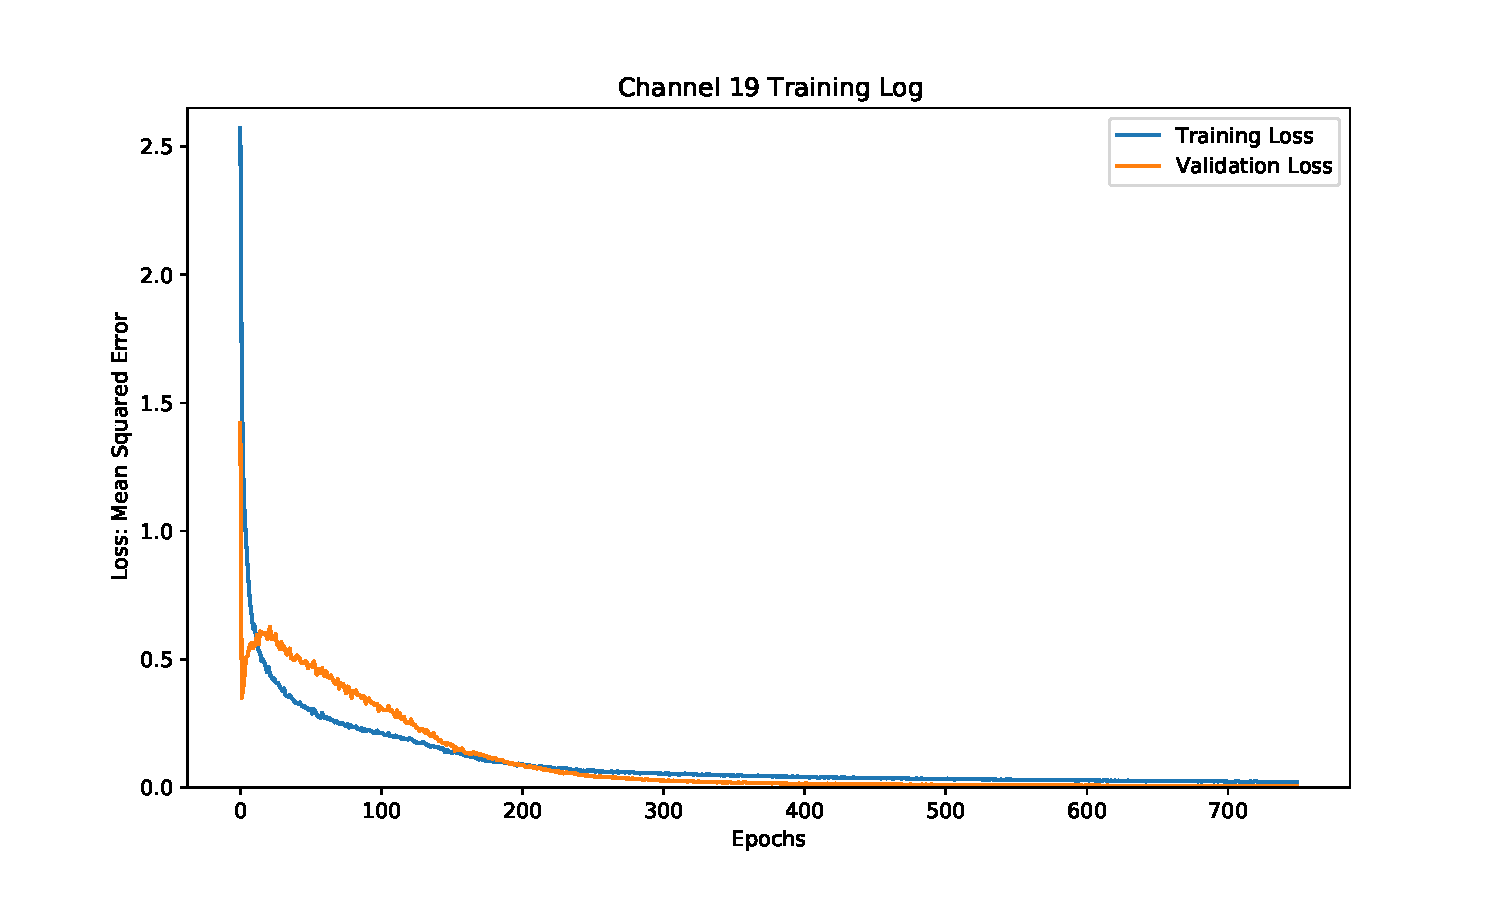
\includegraphics[width=\textwidth]{project/img/ml_model/discrete/Channel 19 Training Log.pdf}
     \end{subfigure}
     \vspace{-4em}
     \begin{subfigure}[b]{\textwidth}
         \centering
         \caption{Epochs 100 to 750.}
         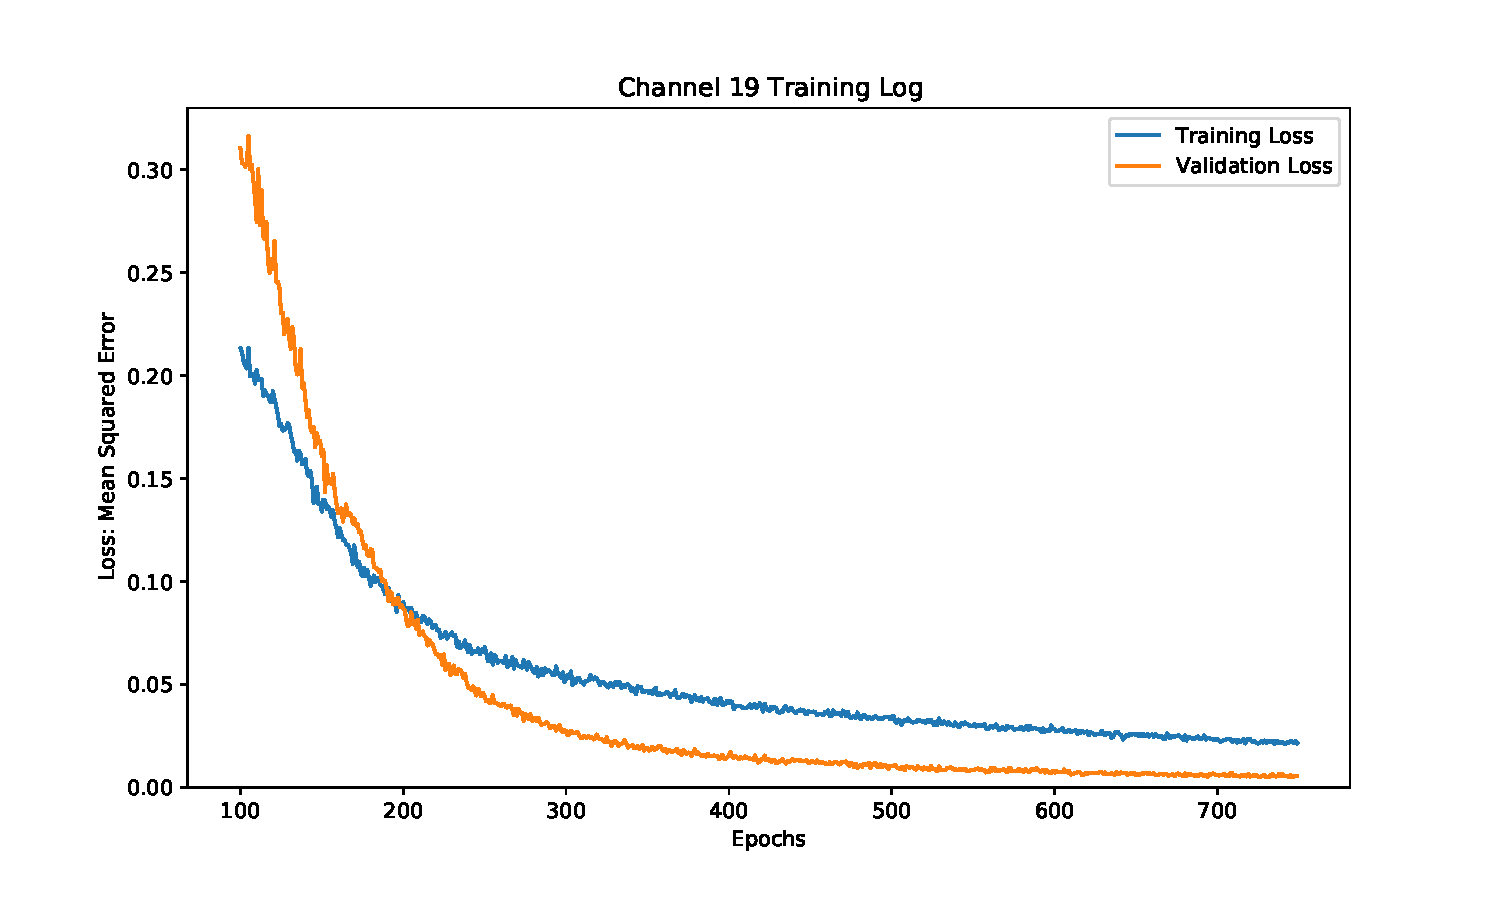
\includegraphics[width=\textwidth]{project/img/ml_model/discrete/Channel 19 Training Loginset.pdf}
     \end{subfigure}
        \label{fig:ml_model:disc_train_log}
\end{figure}

% Include a picture of a training graph for the model

\begin{figure}
    \centering
    \caption{MPE of each Neural Network after training for 750 epochs, training is show in orange and validation is shown in blue.}
    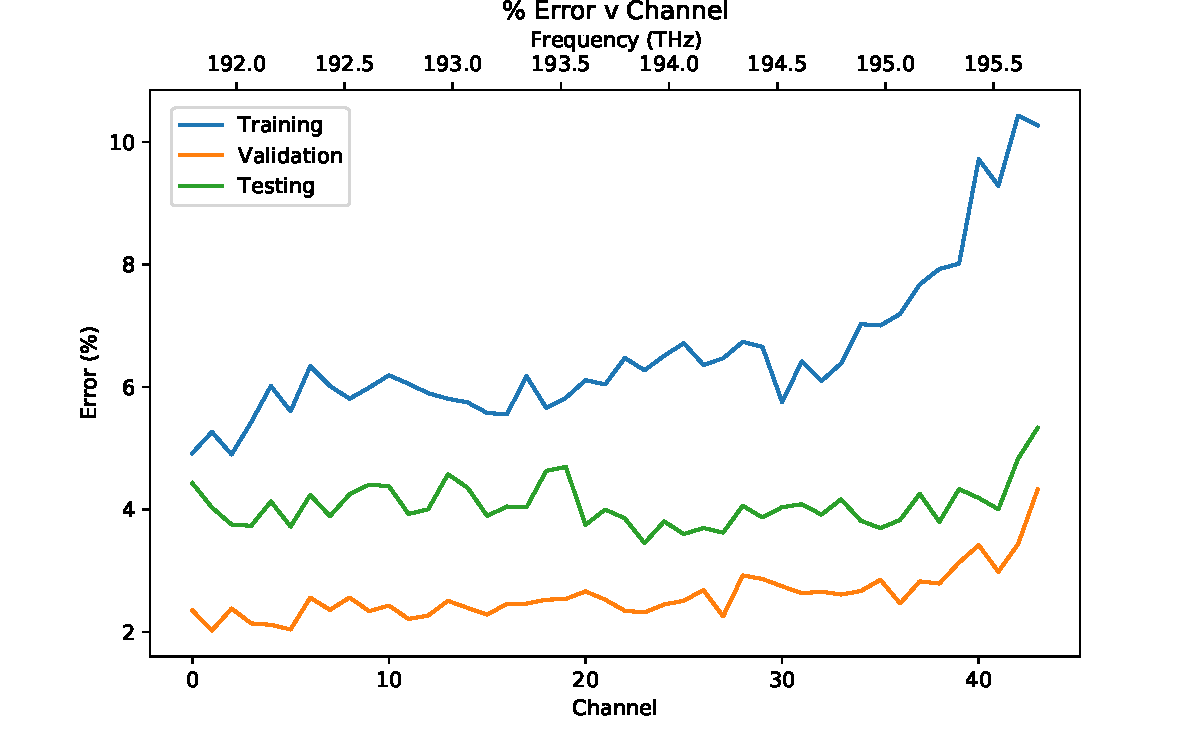
\includegraphics[width=\textwidth]{project/img/ml_model/discrete/percent_error.pdf}
    \label{fig:ml_model:disc_train_val}
\end{figure}

\FloatBarrier
\subsection{Model Configuration}

\FloatBarrier
\subsubsection{Optimiser}
The Nadam optimiser was used to train the model. The choice of optimiser was made based on a series of experiments, training representative sample models.  
\begin{figure}
    \centering
    \caption{Convergence of Nadam optimiser v Stochastic Gradient Decent, for channel 19}
    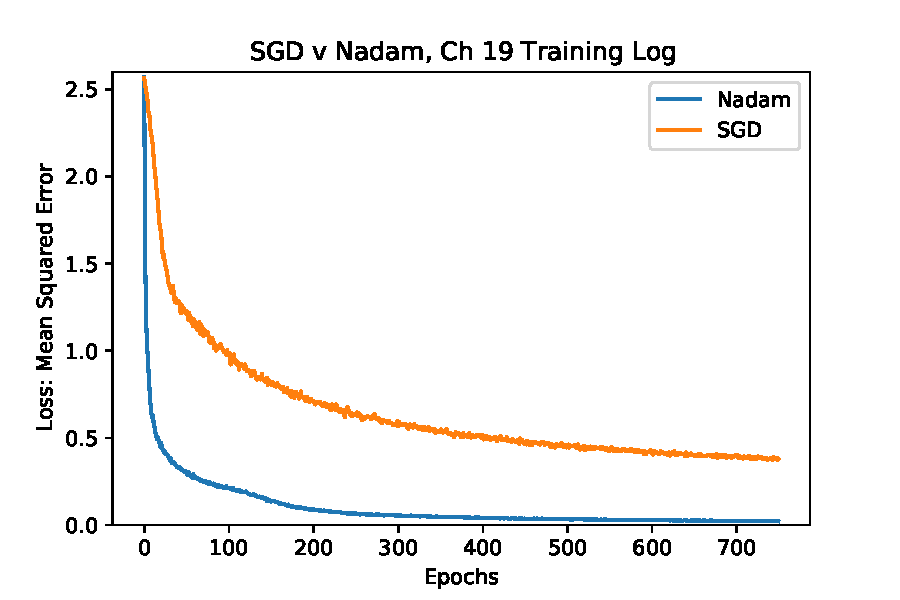
\includegraphics[width=\textwidth]{project/img/ml_model/discrete/SGD v Nadam, Ch 19 Training Log.pdf}
    \label{fig:ml_model:sgd_nadam}
\end{figure}

\FloatBarrier
\subsubsection{Loss Function}
\FloatBarrier
\begin{figure}
    \centering
    \caption{Comparison of Mean Squared Error v Mean Absolute Percentage Error loss functions.}
    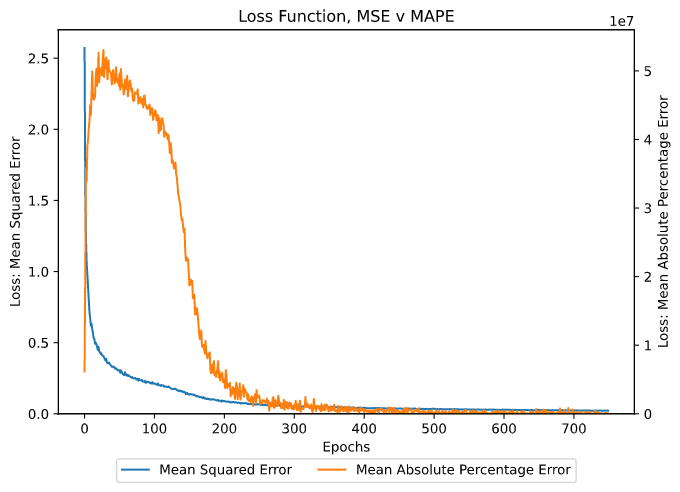
\includegraphics[width=\textwidth]{project/img/ml_model/discrete/mse_mpe.png}
    \label{fig:ml_model:mse_mpe}
\end{figure}

\FloatBarrier
\subsubsection{Activation function}


\subsection{Conclusion}

\chapter{Evaluation}
\chapter{Conclusion}
\bibliographystyle{unsrtnat}
\bibliography{bibs/sample}
\appendix
\renewcommand{\thechapter}{A\arabic{chapter}}
\chapter{Appendix}
You may use appendices to include relevant background information, such as calibration certificates, derivations of key equations or presentation of a particular data reduction method. You should not use the appendices to dump large amounts of additional results or data which are not properly discussed. If these results are really relevant, then they should appear in the main body of the report.

\section{Appendix numbering}
Appendices are numbered sequentially, A1, A2, A3\ldots The sections, figures and tables within appendices are numbered in the same way as in the main text. For example, the first figure in Appendix A1 would be Figure A1.1. Equations continue the numbering from the main text.



\end{document}